\par\Needspace{10\baselineskip}
\section{曲面积分}
\label{sec:analysis-surface-integration}

路径积分沿一条细线累计：线密度乘弧长得到质量，力与位移的内积累加得到做功。
曲面积分把累计的范围从细线换成薄片，典型问题有两个。
第一个问题是求一张金属薄壳的质量：已知壳上每点每平方米有多少千克，把各小片的“面密度乘面积”加起来即可。
第二个问题是求单位时间内有多少水穿过一张渔网：水在各点有速度，只有垂直于网面的速度分量才把水送到网的另一侧。

两个问题的被积对象不同。
在第一个问题中，被积对象是曲面$S$上的标量函数$h:S\to\mathbb R$，它给出每单位面积的密度，乘面积后相加得到质量、电荷等总量。
在第二个问题中，被积对象是向量场$\bm F:S\to\mathbb R^3$，它在每点给出一个有大小和方向的量；要先取它垂直于曲面的分量，再乘面积相加，得到穿过曲面的\emph{通量}。

两类积分都需要知道曲面上一小片有多大，所以本节先用参数化求出面积元。
通量还需要规定“从哪一侧穿到哪一侧算正”，因此在定义第二类积分之前，还要讨论曲面的定向。
本节的积分都按勒贝格积分理解；参数曲面、面积元和通量的标准构造可参考\scite{math-openstax-calculus3}。

\subsection{参数曲面与面积}

平面区域的面积就是它的二维勒贝格测度。
空间中的曲面一般是弯曲的，不能不经伸缩地摊平成平面区域，所以不能直接用二维测度计算它的面积。
处理地球表面时，人们用经度和纬度两个数确定地面上的一点，这就是一种参数化：用两个参数标记曲面上的点，把曲面上的累计转回二维参数域上计算。
代价是参数域中的面积一般不等于曲面上的实际面积。
经纬度网格上同样大小的格子，在赤道附近和两极附近对应的实际地面面积并不相同，因此每一点都要乘一个面积放大倍数来校正。
本小节先说明怎样的参数化才能描述一张面，再求出这个放大倍数，并证明由此得到的面积不依赖参数的选取。

\subsubsection{曲面的参数化}

\paragraph{正则曲面片}

曲面的参数化是一个向量值映射：输入两个实数$(u,v)$，输出空间中一点的三个坐标。
并不是每个这样的映射都描述一张面。
若改变两个参数时点只沿同一个方向移动，像集可能只是一条曲线；
若不同参数在一块正面积的范围内对应同一些点，按参数累计就会把这块面计算两次。
下面的定义用正则性和单次覆盖两个条件分别排除这两种情况。

\begin{definition}[正则参数曲面片]
\label{def:analysis-regular-surface-patch}
设$E\subseteq\mathbb R^2$是有界闭区域，$E=\overline{E^\circ}$且二维勒贝格测度$m_2(\partial E)=0$。
设$\bm r$在$E$的一个开邻域内是$C^1$映射，写成
\[
 \bm r(u,v)=(x(u,v),y(u,v),z(u,v))^\top\in\mathbb R^3.
\]
若不同参数只有在都属于$\partial E$时才允许表示同一点，
且两个偏导向量$\bm r_u,\bm r_v$在$E^\circ$上处处线性无关，则称$\bm r$为一个正则曲面片的参数化，曲面片记为$S=\bm r(E)$。
参数边界允许产生接缝或退化点；这些边界部分按零曲面面积处理。
\end{definition}

定义中的两个偏导向量有直接的几何含义。
固定$v$而只改变$u$，点$\bm r(u,v)$在曲面上画出一条参数曲线，它的速度向量是$\bm r_u$；
固定$u$而改变$v$得到另一条参数曲线，速度向量是$\bm r_v$。
这里$\bm r_u,\bm r_v$都是三维向量，分别由三个坐标函数对同一个参数求偏导得到，并非某个标量函数的两个偏导数。

两个向量线性无关，是指对任意实数$\alpha,\beta$，
$\alpha\bm r_u+\beta\bm r_v=\bm0$只有在$\alpha=\beta=0$时才成立。
几何上，这表示两个向量不共线，它们张成过该点的一个平面，即曲面的切平面。
若这个条件不成立，像集可能根本不是一张面。

\begin{example}[像集退化为线段的参数映射]
取$E=[0,1]^2$和$\bm r(u,v)=(u+v,0,0)^\top$。
两个偏导向量都等于$(1,0,0)^\top$，因而线性相关。
当$(u,v)$取遍$E$时，$u+v$取遍$[0,2]$，所以像集是$x$轴上的线段$\{(x,0,0)^\top:0\leq x\leq2\}$。
整个正方形被压到这条线段上，像集上没有两个不共线的切方向，也没有面积可言；这个映射不满足正则性条件。
\end{example}

正则性条件排除了这种压扁的映射。
单次覆盖条件处理另一种情况：像集确实是一张面，但被参数重复计数。

\begin{example}[圆柱面的单次覆盖与二重覆盖]
\label{ex:analysis-cylinder-double-cover}
高为$1$的单位圆柱面可以写成
\[
 \bm r(\theta,z)=(\cos\theta,\sin\theta,z)^\top,\qquad z\in[0,1].
\]
偏导向量$\bm r_\theta=(-\sin\theta,\cos\theta,0)^\top$与$\bm r_z=(0,0,1)^\top$处处线性无关，正则性没有问题，需要检查的只有覆盖次数。
若$\theta\in[0,2\pi]$，只有$\theta=0$与$\theta=2\pi$两条边界线表示同一条接缝，这是定义允许的。
若$\theta\in[0,4\pi]$，则对$0<\theta_0<2\pi$和$0<z<1$，点$\bm r(\theta_0,z)$同时由参数域内部的$(\theta_0,z)$和$(\theta_0+2\pi,z)$表示；
按参数累计会把整张柱面计入两次，因此这一参数域不符合定义。
\end{example}

所以不同参数表示同一点的情形只允许出现在参数边界上，形成接缝；参数域内部的点不能与任何其他参数点表示同一点。

本小节反复使用的例子是$\bm r(u,v)=(u,v,u+v)^\top$、$E=[0,1]^2$，下文称它为斜平面片。
它描述平面$z=x+y$上位于单位正方形上方的一块平行四边形，
两个切向量分别为$\bm r_u=(1,0,1)^\top$和$\bm r_v=(0,1,1)^\top$。
前两个坐标就是参数本身，所以不同参数给出不同点；两个切向量不共线，所以它满足正则曲面片的定义。

\paragraph{叉积}

要求曲面的面积，先看参数域中的一个小矩形$[u,u+\Delta u]\times[v,v+\Delta v]$被映成什么形状。
由$\bm r$的可微性，在$\Delta u,\Delta v$很小时有线性近似
\[
 \bm r(u+\Delta u,v+\Delta v)\approx\bm r(u,v)+\bm r_u\Delta u+\bm r_v\Delta v,
\]
其中$\bm r,\bm r_u,\bm r_v$都在$(u,v)$处取值。
于是小矩形的四个顶点近似映为
$\bm r$、$\bm r+\bm r_u\Delta u$、$\bm r+\bm r_v\Delta v$和$\bm r+\bm r_u\Delta u+\bm r_v\Delta v$，
它们正是以$\bm r_u\Delta u$和$\bm r_v\Delta v$为两边的平行四边形的顶点。
所以曲面上的小片近似是切平面内的一个小平行四边形，问题归结为：怎样由两条边向量求平行四边形的面积。

在平面上，两个边向量排成$2\times2$矩阵，其行列式的绝对值就是这个面积。
现在两条边是三维向量，排成的是$3\times2$矩阵，没有行列式可取。
三维空间中常用叉积同时记录这个面积和平行四边形所在平面的垂直方向。
对$\bm a,\bm b\in\mathbb R^3$，定义叉积
\[
 \bm a\times\bm b
 =(a_2b_3-a_3b_2,\ a_3b_1-a_1b_3,\ a_1b_2-a_2b_1)^\top.
\]
例如$(1,0,0)^\top\times(0,1,0)^\top=(0,0,1)^\top$：
$x$轴方向与$y$轴方向的单位向量张成面积为$1$的正方形，叉积是长度为$1$、沿$z$轴的向量。

后面的面积和法向计算要用到叉积的三条性质，下面逐一核对。
第一，叉积垂直于$\bm a$和$\bm b$。直接展开
\[
 \bm a^\top(\bm a\times\bm b)
 =a_1(a_2b_3-a_3b_2)+a_2(a_3b_1-a_1b_3)+a_3(a_1b_2-a_2b_1),
\]
右端六项两两抵消，结果为$0$；对$\bm b$同理。
垂直于同一平面的方向有相反的两个，叉积按右手规则选取其中之一：右手四指从$\bm a$弯向$\bm b$时，拇指指向$\bm a\times\bm b$。

第二，叉积的长度等于$\bm a,\bm b$张成的平行四边形的面积。
把两边按分量展开，可以验证Lagrange恒等式
\[
 \lVert\bm a\times\bm b\rVert_2^2
 =\lVert\bm a\rVert_2^2\lVert\bm b\rVert_2^2-(\bm a^\top\bm b)^2.
\]
记$\theta\in[0,\pi]$为两向量的夹角，则$\bm a^\top\bm b=\lVert\bm a\rVert_2\lVert\bm b\rVert_2\cos\theta$，
代入得$\lVert\bm a\times\bm b\rVert_2=\lVert\bm a\rVert_2\lVert\bm b\rVert_2\sin\theta$。
以$\bm a$为底边时，平行四边形的高是$\lVert\bm b\rVert_2\sin\theta$，所以叉积长度正是“底乘高”。
特别地，叉积为零当且仅当两向量共线，即平行四边形退化为线段或一点。

第三，叉积对每个因子都是线性的，交换两个因子的次序会变号：从定义式直接看出$\bm b\times\bm a=-\bm a\times\bm b$，特别地$\bm a\times\bm a=\bm0$。
这与右手规则一致：交换次序后四指的弯曲方向相反，拇指也随之反向。

把这些性质用到小平行四边形上。由线性，
$(\bm r_u\Delta u)\times(\bm r_v\Delta v)=(\bm r_u\times\bm r_v)\Delta u\Delta v$；
再由第二条性质，小曲面片的面积近似为
\[
 \lVert\bm r_u\times\bm r_v\rVert_2\,\Delta u\,\Delta v.
\]
因此$\lVert\bm r_u\times\bm r_v\rVert_2$就是参数化在该点的面积放大倍数：参数域中面积为$\Delta u\Delta v$的小块，
在曲面上变成面积约为这个倍数乘$\Delta u\Delta v$的小片。
同样由第二条性质，正则性条件“两个切向量线性无关”可以等价地写成$\bm r_u\times\bm r_v\ne\bm0$，即放大倍数处处为正。

平面情形可以用来核对这个倍数。若曲面就在平面$z=0$内，即$\bm r(u,v)=(x(u,v),y(u,v),0)^\top$，
则$\bm r_u\times\bm r_v=(0,0,x_uy_v-x_vy_u)^\top$，其长度正是映射$(u,v)\mapsto(x,y)$的Jacobian行列式的绝对值。
这与第~\ref{sec:multivariable-change-variables}节换元公式中的面积权重$|\det\bm J_T|$一致；叉积长度是这个权重在三维空间中的推广。

\subsubsection{曲面面积的表示}

\paragraph{面积元与面积测度}

把参数域分成许多小矩形，由小平行四边形的面积近似，每块在曲面上的像的面积约为放大倍数乘参数面积，曲面的总面积约为这些乘积之和。
小矩形越细，线性近似越准确，求和的极限就是放大倍数在参数域上的积分。

这里直接把这个积分取作曲面面积的定义，而不像弧长那样用内接折线长度的上确界来定义，因为曲面上的类似做法会失败。
在一段有限高的圆柱面上，可以构造顶点都在柱面上的三角形网格（称为Schwarz灯笼），
使网格越来越细，三角形与柱面的夹角却不趋于零，三角形总面积可以趋于无穷。
用切平面上的平行四边形近似则不会出现这种问题，因为每个小平行四边形都贴着切平面。

\begin{definition}[曲面面积测度]
\label{def:analysis-surface-area-measure}
在上述曲面片上，记$J_S(u,v)=\lVert\bm r_u\times\bm r_v\rVert_2$。
若$A\subseteq S$的原像$\bm r^{-1}(A)\cap E$勒贝格可测，则称$A$为曲面可测集，定义
\[
 \sigma_S(A)=\iint_E\bm1_A(\bm r(u,v))J_S(u,v)\,\mathrm du\,\mathrm dv.
\]
曲面面积元记为$\mathrm dS$，参数表示为
\[
 \mathrm dS=J_S(u,v)\,\mathrm du\,\mathrm dv,
 \qquad \operatorname{area}(S)=\sigma_S(S).
\]
\end{definition}

$\sigma_S(A)$先找出$A$在参数域中的原像，再把原像上每一点的放大倍数积起来。
这样得到的确实是一个测度。原像运算保持集合的补、交和可数并，所以曲面可测集构成$\sigma$代数。
对两两不交的曲面可测集，并集的指示函数等于各指示函数之和；$\sigma_S$由非负函数的勒贝格积分给出，由单调收敛定理（定理~\ref{thm:analysis-monotone-convergence}）可以逐项积分，所以$\sigma_S$可数可加。

$J_S$在紧集$E$上连续，因而有界；又$m_2(E)<\infty$，故曲面片的面积有限。
参数边界的二维测度为零，在定义式中不贡献面积；边界接缝上的点即使被两个参数表示，也只位于零测集上，不会造成正面积的重复累计。

用这一定义计算斜平面片的面积，并用初等几何核对结果。

\begin{example}[斜平面片的面积]
\label{ex:analysis-tilted-plane-area}
对斜平面片$\bm r(u,v)=(u,v,u+v)^\top$、$E=[0,1]^2$，按叉积的定义计算
\[
 \begin{aligned}
 \bm r_u\times\bm r_v
 &=(1,0,1)^\top\times(0,1,1)^\top\\
 &=(0\cdot1-1\cdot1,\ 1\cdot0-1\cdot1,\ 1\cdot1-0\cdot0)^\top
 =(-1,-1,1)^\top,
 \end{aligned}
\]
故$J_S=\lVert(-1,-1,1)^\top\rVert_2=\sqrt3$处处成立，曲面面积为
\[
 \operatorname{area}(S)=\int_0^1\int_0^1\sqrt3\,\mathrm du\,\mathrm dv=\sqrt3.
\]
用初等几何核对：两条边$\bm r_u,\bm r_v$的长度都是$\sqrt2$，内积为$1$，夹角余弦为$1/2$，即夹角为$60^\circ$；
平行四边形面积为$\sqrt2\cdot\sqrt2\cdot\sin60^\circ=\sqrt3$，与积分结果相同。
\end{example}

参数正方形的面积只有$1$，曲面片的面积却是$\sqrt3$：每个参数小块都被放大$\sqrt3$倍。
图~\ref{fig:analysis-process-surface-area-stretch}将参数小块与实际斜面小块对应起来，显示叉积长度校正的是哪一个面积。
\begin{figure*}[!htbp]
 \centering
 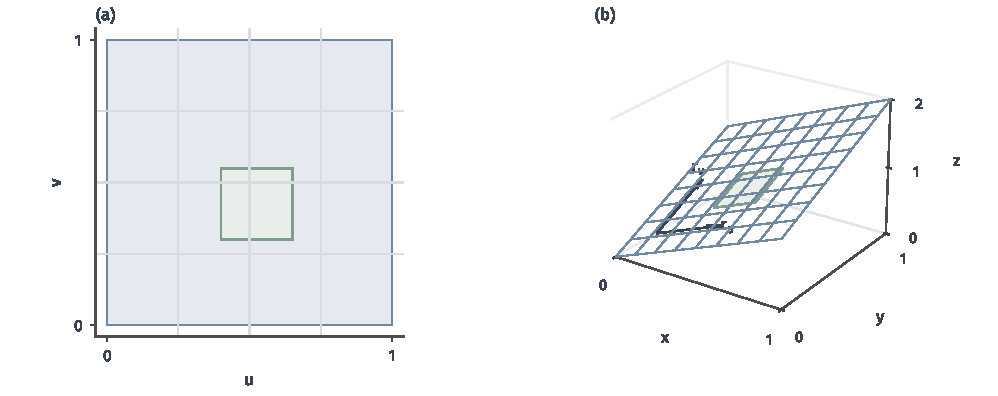
\includegraphics[width=169.0mm]{figures/00-shared/mathematical-preliminaries-upper/00-shared/matplotlib/chapter3-concept-processes/surface-area-stretch.pdf}
 \caption{参数化$r(u,v)=(u,v,u+v)^\top$把单位正方形映为斜平面片，绿色块为同一参数子区间及其像。两切向量$r_u=(1,0,1)^\top$、$r_v=(0,1,1)^\top$在右侧按$0.4$倍画出，叉积长度为$\sqrt3$。每个参数面积都放大$\sqrt3$倍，故不能把$\mathrm du\,\mathrm dv$直接当成$\mathrm dS$。}
 \label{fig:analysis-process-surface-area-stretch}
\end{figure*}

\paragraph{重参数化}

同一张面可以用不同参数标记。
面积是曲面本身的属性，不应随标记方式改变；先在斜平面片上核对一次具体的换参数。

\begin{example}[拉伸一个参数不改变面积]
\label{ex:analysis-stretched-parameter-area}
在斜平面片中令$u=2\xi$，则
\[
 \widetilde{\bm r}(\xi,v)=(2\xi,v,2\xi+v)^\top,\qquad (\xi,v)\in[0,1/2]\times[0,1]
\]
描述同一块平行四边形，新参数域的面积只有$1/2$。
另一方面，$\widetilde{\bm r}_\xi=(2,0,2)^\top=2\bm r_u$，$\widetilde{\bm r}_v=\bm r_v$，由叉积的线性，
$\widetilde{\bm r}_\xi\times\widetilde{\bm r}_v=2(\bm r_u\times\bm r_v)=2(-1,-1,1)^\top$，放大倍数为$2\sqrt3$。
因此
\[
 \int_0^1\int_0^{1/2}2\sqrt3\,\mathrm d\xi\,\mathrm dv=\sqrt3,
\]
与示例~\ref{ex:analysis-tilted-plane-area}的结果相同。
\end{example}

参数域缩小一半，每点的放大倍数恰好加倍，两者相互抵消。
下面的定理说明，这种抵消对一般的单次覆盖换参数都成立。

\begin{theorem}[重参数化下的面积元]
\label{thm:analysis-surface-reparameterization}
设$\bm r:E\to S$是正则曲面片的参数化，$T:\widetilde E\to E$是参数域之间的双射，
在$\widetilde E$的一个开邻域内为$C^1$映射，并且限制在$\widetilde E^\circ$上是到$E^\circ$的$C^1$微分同胚。
若$\widetilde{\bm r}=\bm r\circ T$仍满足曲面片条件，则
\[
 \begin{aligned}
 \widetilde{\bm r}_\xi\times\widetilde{\bm r}_\eta
 &=\det\bm J_T\,(\bm r_u\times\bm r_v)\circ T,\\
 \widetilde J_S&=(J_S\circ T)|\det\bm J_T|.
 \end{aligned}
\]
两组参数由此给出同一面积测度。
\end{theorem}

\begin{proof}
记$T(\xi,\eta)=(u(\xi,\eta),v(\xi,\eta))$。
链式法则给出$\widetilde{\bm r}_\xi=\bm r_u u_\xi+\bm r_v v_\xi$和
$\widetilde{\bm r}_\eta=\bm r_u u_\eta+\bm r_v v_\eta$，其中右端各量在$T(\xi,\eta)$处取值。
用叉积对每个因子的线性展开，得到四项：
\[
 \begin{aligned}
 \widetilde{\bm r}_\xi\times\widetilde{\bm r}_\eta
 &=u_\xi u_\eta(\bm r_u\times\bm r_u)+u_\xi v_\eta(\bm r_u\times\bm r_v)\\
 &\quad{}+v_\xi u_\eta(\bm r_v\times\bm r_u)\\
 &\quad{}+v_\xi v_\eta(\bm r_v\times\bm r_v).
 \end{aligned}
\]
由$\bm a\times\bm a=\bm0$，第一、四项为零；交换叉积次序会变号，即$\bm r_v\times\bm r_u=-\bm r_u\times\bm r_v$，于是第三项可与第二项合并。因此
\[
 \widetilde{\bm r}_\xi\times\widetilde{\bm r}_\eta
 =(u_\xi v_\eta-v_\xi u_\eta)(\bm r_u\times\bm r_v)\circ T,
\]
括号内正是$\det\bm J_T$，这就是第一式；两边取长度得到第二式。
对任一可测集$A\subseteq S$，新参数下的面积为
\[
 \iint_{\widetilde E}\bm1_A(\bm r(T(\xi,\eta)))\,J_S(T(\xi,\eta))\,|\det\bm J_T(\xi,\eta)|\,\mathrm d\xi\,\mathrm d\eta.
\]
在$\widetilde E^\circ$上应用二维换元公式~\eqref{eq:measurable-change-variables}，并注意参数边界为零测集，
它等于$\iint_E\bm1_A(\bm r(u,v))J_S(u,v)\,\mathrm du\,\mathrm dv$，即原参数下的面积。
\end{proof}

几何上，这个证明把两步面积放大接在一起：新参数的小方块先由$T$映成原参数域中面积约为$|\det\bm J_T|$倍的小块，
这个小块再由$\bm r$映到曲面，面积又乘$J_S$。
二维换元公式恰好把第一步的倍数吸收掉，所以只剩下曲面本身的面积。
在示例~\ref{ex:analysis-stretched-parameter-area}中，$T(\xi,v)=(2\xi,v)$，$\det\bm J_T=2$，这正是放大倍数加倍的来源。

行列式的绝对值保证面积非负；行列式本身的符号则记录参数次序是否翻转。
例如在斜平面片上交换两个参数，令$T(\xi,\eta)=(\eta,\xi)$，即$\widetilde{\bm r}(\xi,\eta)=\bm r(\eta,\xi)=(\eta,\xi,\xi+\eta)^\top$，则$\det\bm J_T=-1$，
叉积由$(-1,-1,1)^\top$变为$(1,1,-1)^\top$，长度不变而方向相反。
面积不使用这个方向，后面选取通量的法向时则要用到它。

定理还要求$T$是双射。若参数在正面积的范围内重复覆盖，参数积分就会重复累计。
示例~\ref{ex:analysis-cylinder-double-cover}中，$\bm r_\theta\times\bm r_z=(\cos\theta,\sin\theta,0)^\top$，$J_S=1$；
$\theta\in[0,2\pi]$时参数积分给出柱面面积$2\pi$，$\theta\in[0,4\pi]$时却给出$4\pi$，不能当作单次覆盖的曲面面积。

\paragraph{分片曲面}

有些曲面不能用一张正则曲面片描述。单位立方体的表面由六个正方形组成，棱上没有切平面。
球面虽然可以用一张球坐标参数片覆盖（两极位于参数边界上，切向量在那里退化），也常分成上下两个半球分别处理。
本节只处理有限分片的情形：把曲面写成有限张正则曲面片的并，各片内部不重叠，交接部分在相邻曲面片中面积均为零，
整个曲面的面积测度由各片的面积测度相加。

例如立方体表面的面积就是六个单位正方形的面积之和$6$，十二条棱的面积为零，不需要在接缝上另加一项。
后面的两类曲面积分同样可以逐片计算再相加。
无界曲面，或不能这样由有限张正则曲面片覆盖的曲面，还需另外处理覆盖和可积性条件。

\subsection{第一类曲面积分}

有了面积测度，就可以回到本节开头的第一个问题：在曲面上累计一个标量密度。
这类积分只用到小片的面积，不涉及方向。

\subsubsection{积分的定义和可积性}

\paragraph{按面积的积分}

设一张薄金属壳占据曲面$S$，在点$\bm x$附近每单位面积的质量为$h(\bm x)$（单位如千克每平方米）。
把壳分成许多小片$S_j$，在每片内取一点$\bm x_j$。
若每片很小，片内面密度近似为常数$h(\bm x_j)$，这一片的质量约为$h(\bm x_j)\,\sigma_S(S_j)$。
把各片质量相加，再让分割越来越细，就得到面密度对面积测度的积分。
带电薄壳上的电荷量、涂层表面的涂料用量都是同一种累计。
下面的定义直接使用面积测度上的勒贝格积分，因此不仅适用于连续密度，也适用于有跳跃或仅可测的密度。

\begin{definition}[第一类曲面积分]
\label{def:analysis-scalar-surface-integral}
设$h$是$S$上的可测标量函数。
当$h\geq0$时，定义它的\term{第一类曲面积分}（scalar surface integral）为
\begin{equation}
 \int_Sh\,\mathrm dS
 =\iint_Eh(\bm r(u,v))J_S(u,v)\,\mathrm du\,\mathrm dv.
 \label{eq:analysis-scalar-surface-integral}
\end{equation}
该值允许为$+\infty$。一般实值$h$在$\int_S|h|\,\mathrm dS<\infty$时称为曲面可积，
其积分按正、负部分之差定义，仍满足上式。
\end{definition}

式~\eqref{eq:analysis-scalar-surface-integral}右端的计算顺序是：用参数找到曲面上的点，读出该点的密度，乘该点的面积放大倍数，再在参数域上积分。
定理~\ref{thm:analysis-surface-reparameterization}表明两组单次覆盖的正则参数给出同一面积测度，所以换用另一组参数不会改变积分值。
取$h=1$得到面积，取非负面密度得到质量。
例如在斜平面片上，常数密度$h=2$给出
\[
 \int_S2\,\mathrm dS=\int_0^1\int_0^1 2\sqrt3\,\mathrm du\,\mathrm dv=2\sqrt3,
\]
即面积为$\sqrt3$、每单位面积重$2$的薄片，总质量为$2\sqrt3$。

除了总量，第一类积分还给出曲面上的平均值。设$0<\operatorname{area}(S)<\infty$且$h$曲面可积，则
\[
 \frac1{\operatorname{area}(S)}\int_Sh\,\mathrm dS
\]
是$h$按面积加权的平均。若$h$表示地球表面各点的气温，这个量就是全球表面平均气温：
每块地面按其实际面积参与平均，而不是按经纬度网格的格子数参与平均。

质量和平均值都只依赖每小片的大小，不依赖从哪一侧看曲面，所以把曲面的朝向反过来，第一类积分不变。

\paragraph{可积性的要求}

对一般实值函数，第一类积分要求绝对积分有限。
由定义，$h$曲面可积当且仅当$h\circ\bm r$在$E$上可测，且
\[
 \iint_E|h(\bm r(u,v))|J_S(u,v)\,\mathrm du\,\mathrm dv<\infty,
\]
也就是函数大小乘面积权重后在参数域上的累计有限。
连续函数是一个便于验证的充分情形：$S=\bm r(E)$紧致，连续的$h$在其上有界，
因而$\int_S|h|\,\mathrm dS\leq \sup_S|h|\,\sigma_S(S)<\infty$。

可测性本身并不保证绝对积分有限。
函数在某点附近无界时，要比较它增大的速度与该点附近面积缩小的速度。
下面以球面上到北极点距离的负幂为例，先用环带面积估计可积的阈值。

\begin{example}[球面上距离负幂的可积阈值]
\label{ex:analysis-sphere-distance-power}
设$S$是以原点为中心、半径为$R$的球面，$\bm N=(0,0,R)^\top$为北极点，$\alpha>0$，
令$h(\bm x)=\lVert\bm x-\bm N\rVert_2^{-\alpha}$（$\bm N$处任取一值，单点的面积为零）。
在到北极点的距离不小于某个正数的部分，$h$有界，所以问题只在北极点附近。
到北极点距离为$\rho$的点组成一个圆，$\rho$很小时它的周长约为$2\pi\rho$；所以距离介于$\rho$与$\rho+\Delta\rho$之间的环带面积约为$2\pi\rho\,\Delta\rho$，而$h$在环带上约为$\rho^{-\alpha}$。
因此北极附近的累计与
\[
 \int_0^\delta\rho^{-\alpha}\cdot2\pi\rho\,\mathrm d\rho
 =2\pi\int_0^\delta\rho^{1-\alpha}\,\mathrm d\rho
\]
同时有限或同时发散，其中$\delta>0$是某个小数。
右端在$\alpha<2$时有限、在$\alpha\geq2$时发散，所以按这一估计，$h$曲面可积当且仅当$\alpha<2$。
示例~\ref{ex:analysis-sphere-distance-power-exact}将用球坐标精确计算这个积分，验证这里的估计。
\end{example}

这一阈值与平面上$\lVert\bm x\rVert_2^{-p}$在单位圆盘上可积当且仅当$p<2$的结论（第~\ref{sec:multivariable-riemann-lebesgue}节）相同。
原因是曲面在小范围内近似于切平面，环带面积与平面圆环面积按同样的方式随半径变化。
取$\alpha=1$：电学中点电荷的电势与距离成反比，若点电荷位于北极点，电势在球面上的积分有限。

这些条件都相对于曲面面积而言，而非三维体积测度。
曲面在三维空间中的体积为零，若对三维勒贝格测度积分，任何函数在曲面上的积分都是零；面积测度正是为了给这种零体积集合赋予有意义的大小。

\subsubsection{积分的性质}

第一类曲面积分是面积测度上的勒贝格积分，因此勒贝格积分的线性、可加性和单调性都直接适用。
以下各条均以相应函数曲面可积为前提，并分别说明它们在薄壳质量或电荷上的含义。

\paragraph{加法}

对曲面可积的$h,k$，$h+k$也可积，而且
\[
 \int_S(h+k)\,\mathrm dS=\int_Sh\,\mathrm dS+\int_Sk\,\mathrm dS.
\]
可积性由$|h+k|\leq|h|+|k|$得到，等式来自标量勒贝格积分的加法性质。
若薄壳由两层材料叠成，面密度分别为$h$和$k$，这个等式表示总质量等于两层质量之和。

\paragraph{减法}

对曲面可积的$h,k$，$h-k$也可积，而且
\[
 \int_S(h-k)\,\mathrm dS=\int_Sh\,\mathrm dS-\int_Sk\,\mathrm dS.
\]
这里$|h-k|\leq|h|+|k|$保证绝对可积，等式来自标量勒贝格积分的减法性质。

\paragraph{数乘}

对实数$c$和曲面可积的$h$，$ch$曲面可积，且
\[
 \int_Sch\,\mathrm dS=c\int_Sh\,\mathrm dS.
\]
因为$|ch|=|c||h|$，绝对积分仍有限；等式来自标量勒贝格积分的数乘性质。
例如把面密度的单位从千克每平方米换成克每平方米，相当于$c=1000$，总质量的数值也乘$1000$。

\paragraph{曲面分割的可加性}

若可测子集$A_j\subseteq S$（$j=1,2,\ldots$）两两不交，且$h$在$S$上曲面可积，则
\[
 \int_{\bigcup_{j=1}^\infty A_j}h\,\mathrm dS
 =\sum_{j=1}^\infty\int_{A_j}h\,\mathrm dS.
\]
右侧级数绝对收敛，因为其各项绝对值之和不超过$\int_S|h|\,\mathrm dS$；等式来自勒贝格积分对积分区域的可数可加性。
它表示把薄壳切成若干块分别称重，再把重量相加，与整块称重的结果相同。
有限分片曲面的逐片求和是这一性质的特例；各片仅在零面积接缝上相交，也不影响等式。

\paragraph{单调性}

若曲面可积的$h,k$满足$h\leq k$在曲面面积意义下几乎处处成立，则
\[
 \int_Sh\,\mathrm dS\leq\int_Sk\,\mathrm dS.
\]
因为$k-h$几乎处处非负，其积分非负，应用减法公式即可得到这一不等式。
这里的“几乎处处”允许忽略零曲面面积的集合，例如有限条曲线；它不以三维体积衡量例外集合，否则整张曲面都会被忽略。

\paragraph{绝对值不等式}

对任一曲面可积的$h$，将单调性应用于$-|h|\leq h\leq|h|$得到
\[
 \left|\int_Sh\,\mathrm dS\right|\leq\int_S|h|\,\mathrm dS.
\]
当$h$有正有负时，例如表示正负电荷的面密度，左端是净电荷的大小，右端是不计符号的电荷总量；
正负部分会相互抵消，所以净量不超过总量。

\subsubsection{积分的计算}

计算第一类曲面积分分三步：选一个单次覆盖的正则参数化，把$h$与参数化复合，再乘叉积的长度后在参数域上积分。
最常见的两种参数化是函数图像和球坐标。

若曲面是函数$z=\psi(x,y)$在区域$D$上的图像，其中$D$满足定义~\ref{def:analysis-regular-surface-patch}对参数域的要求，$\psi$在$D$的开邻域内为$C^1$，就可以取
$\bm r(x,y)=(x,y,\psi(x,y))^\top$。此时$\bm r_x=(1,0,\psi_x)^\top$、$\bm r_y=(0,1,\psi_y)^\top$，按叉积公式计算得
\[
 \begin{aligned}
 \bm r_x\times\bm r_y
 &=(0\cdot\psi_y-\psi_x\cdot1,\ \psi_x\cdot0-1\cdot\psi_y,\ 1\cdot1-0\cdot0)^\top\\
 &=(-\psi_x,-\psi_y,1)^\top.
 \end{aligned}
\]
叉积的第三分量恒为$1$，所以图像参数化处处正则；前两个坐标就是参数本身，所以单次覆盖也自动成立。
于是对曲面可积的$h$有
\[
 \int_Sh\,\mathrm dS
 =\iint_Dh(x,y,\psi(x,y))\sqrt{1+\psi_x^2+\psi_y^2}\,\mathrm dx\,\mathrm dy.
\]

根号的几何意义如下。记$\gamma$为法向$(-\psi_x,-\psi_y,1)^\top$与$z$轴的夹角，
则$\cos\gamma=1/\sqrt{1+\psi_x^2+\psi_y^2}$。
一块与水平面成角$\gamma$的小平面片，竖直投影到$xy$平面上时面积缩小为原来的$\cos\gamma$倍；
反过来，由投影面积$\mathrm dx\,\mathrm dy$恢复实际面积，就要除以$\cos\gamma$，即乘上这个根号。
曲面越陡，根号越大。例如$z=ax+by+c$在单位圆盘上方的部分，根号处处等于$\sqrt{1+a^2+b^2}$，面积为
$\pi\sqrt{1+a^2+b^2}$；$a=b=0$时它就是水平圆盘的面积$\pi$。
若曲面不能单值地投影到同一坐标平面，例如整张球面在每个$(x,y)$上方有两点，则需换参数化或分片。

半径$R>0$的球面可以取参数
\[
 \begin{gathered}
 \bm r(\varphi,\theta)
 =(R\sin\varphi\cos\theta,R\sin\varphi\sin\theta,R\cos\varphi)^\top,\\
 0\leq\varphi\leq\pi,\quad 0\leq\theta\leq2\pi,
 \end{gathered}
\]
其中$\varphi$是与北极方向的夹角，$\theta$是绕$z$轴转过的角度。求偏导得
\[
 \begin{aligned}
 \bm r_\varphi&=(R\cos\varphi\cos\theta,R\cos\varphi\sin\theta,-R\sin\varphi)^\top,\\
 \bm r_\theta&=(-R\sin\varphi\sin\theta,R\sin\varphi\cos\theta,0)^\top.
 \end{aligned}
\]
这两个向量的内积为零，长度分别为$R$和$R\sin\varphi$；由叉积长度公式（夹角为$\pi/2$），叉积长度为$R^2\sin\varphi$。
这个结果也可以直接看出：$\varphi$增加$\Delta\varphi$时，点沿经线走过约$R\Delta\varphi$；
$\theta$增加$\Delta\theta$时，点沿半径为$R\sin\varphi$的纬线圈走过约$R\sin\varphi\,\Delta\theta$。
小片近似为以这两个长度为边的矩形。靠近两极时纬线圈变小，同样的$\Delta\theta$对应的面积也变小。

在参数域内部$0<\varphi<\pi$、$0<\theta<2\pi$上$\sin\varphi>0$，参数化正则且单次覆盖；
两极与经线接缝来自参数边界，面积为零，不需要单独处理。
先用这个参数化求球面面积。

\begin{example}[球面的面积]
\label{ex:analysis-sphere-area}
对半径为$R$的球面，球坐标参数的面积放大倍数为$J_S=R^2\sin\varphi$，被积函数非负，可以逐次积分：
\[
 \operatorname{area}(S)
 =\int_0^{2\pi}\int_0^\pi R^2\sin\varphi\,\mathrm d\varphi\,\mathrm d\theta
 =2\pi R^2\bigl[-\cos\varphi\bigr]_0^\pi
 =4\pi R^2.
\]
\end{example}

球坐标也能把示例~\ref{ex:analysis-sphere-distance-power}中的环带估计变成精确计算。

\begin{example}[球面上距离负幂积分的精确值]
\label{ex:analysis-sphere-distance-power-exact}
沿用示例~\ref{ex:analysis-sphere-distance-power}的记号，$\bm N=(0,0,R)^\top$。在球坐标下
\[
 \lVert\bm r(\varphi,\theta)-\bm N\rVert_2^2
 =R^2\sin^2\varphi+R^2(1-\cos\varphi)^2
 =2R^2(1-\cos\varphi)
 =4R^2\sin^2\tfrac\varphi2,
\]
所以到北极点的距离为$s=2R\sin(\varphi/2)$。
它是$\varphi\in[0,\pi]$上递增的$C^1$函数，把$[0,\pi]$映为$[0,2R]$，且$\mathrm ds=R\cos(\varphi/2)\,\mathrm d\varphi$，从而
\[
 R^2\sin\varphi\,\mathrm d\varphi
 =2R^2\sin\tfrac\varphi2\cos\tfrac\varphi2\,\mathrm d\varphi
 =s\,\mathrm ds.
\]
被积函数非负，先对$\theta$积分得到因子$2\pi$，再换元：
\[
 \int_S\lVert\bm x-\bm N\rVert_2^{-\alpha}\,\mathrm dS
 =2\pi\int_0^\pi\Bigl(2R\sin\tfrac\varphi2\Bigr)^{-\alpha}R^2\sin\varphi\,\mathrm d\varphi
 =2\pi\int_0^{2R}s^{1-\alpha}\,\mathrm ds.
\]
当$0<\alpha<2$时，积分值为$2\pi(2R)^{2-\alpha}/(2-\alpha)$；当$\alpha\geq2$时，积分为$+\infty$。
\end{example}

精确结果与环带估计给出同一个阈值。
对$\theta$积分后，面积元成为$2\pi s\,\mathrm ds$，所以到北极点距离介于$s$与$s+\Delta s$之间的环带面积约为$2\pi s\,\Delta s$；这一规律不只在北极附近成立，在整张球面上都成立。

面积权重在求平均时同样不可缺少，下面以上半球面上的平均高度为例。

\begin{example}[上半球面的平均高度]
\label{ex:analysis-hemisphere-average-height}
取上半球面$0\leq\varphi\leq\pi/2$，高度函数$h(\bm x)=z$。
由$J_S=R^2\sin\varphi$，上半球面面积为$2\pi R^2\int_0^{\pi/2}\sin\varphi\,\mathrm d\varphi=2\pi R^2$，而
\[
 \int_Sz\,\mathrm dS
 =\int_0^{2\pi}\int_0^{\pi/2}R\cos\varphi\cdot R^2\sin\varphi\,\mathrm d\varphi\,\mathrm d\theta
 =2\pi R^3\cdot\frac12=\pi R^3,
\]
所以按面积加权的平均高度为$\pi R^3/(2\pi R^2)=R/2$。
若改为在参数矩形$[0,\pi/2]\times[0,2\pi]$上按参数面积平均，则得到
\[
 \frac1{(\pi/2)\cdot2\pi}\int_0^{2\pi}\int_0^{\pi/2}R\cos\varphi\,\mathrm d\varphi\,\mathrm d\theta
 =\frac{2R}{\pi}\approx0.64R.
\]
\end{example}

两种平均不同，是因为同样大小的参数格子在北极附近只对应很小的面积：按参数平均会过多计入北极附近的高点，因而高估平均高度。
面积权重$R^2\sin\varphi$正是为了按实际面积而不是按参数格子求平均。

\subsection{第二类曲面积分}

现在回到本节开头的第二个问题：向量场穿过曲面的总量。
面积测度只给出小片的大小；要说“穿过”，还必须先规定曲面的哪一侧算出发侧、哪一侧算到达侧。
因此本小节先讨论曲面的定向，再定义通量。

\subsubsection{曲面的定向}

\paragraph{单位法向量}

在正则点，切平面有两个互相相反的单位法向量，分别指向曲面的两侧。
选定其中一个，就约定：从曲面上背向它的一侧穿到它所指的一侧，算作正向穿越。
参数化的叉积给出一个自然的局部选择：在$E^\circ$上令
\[
 \bm n(\bm r(u,v))
 =\frac{\bm r_u\times\bm r_v}{\lVert\bm r_u\times\bm r_v\rVert_2}.
\]
由叉积的性质，这个向量长度为$1$，并且垂直于两个参数方向，即垂直于切平面；交换$u,v$的次序会把它反转。

在斜平面片上，这个公式给出$(-1,-1,1)^\top/\sqrt3$，它的第三分量为正，指向平面的上方。
在球坐标参数下，直接计算可得
\[
 \bm r_\varphi\times\bm r_\theta
 =R^2\sin\varphi\,(\sin\varphi\cos\theta,\sin\varphi\sin\theta,\cos\varphi)^\top
 =R\sin\varphi\,\bm r(\varphi,\theta).
\]
在参数域内部，叉积是位置向量的正数倍，所以单位法向为$\bm r/R$，指向球的外侧。
参数边界上若叉积退化，例如球面的两极，就不用这个商定义法向；该部分面积为零，不影响通量积分。

\paragraph{定向与可定向性}

只在每一点分别选一个法向还不够。若相邻两点选的法向分别指向曲面的两侧，“正向穿越”就没有一致的含义。
直观地说，给曲面定向就是给它的一侧涂上颜色，并约定法向总是从未涂色的一侧指向涂了色的一侧；
沿曲面连续移动时，法向箭头不能突然跳到另一侧。

\begin{definition}[曲面的定向]
\label{def:analysis-surface-orientation}
在光滑曲面$S$上连续选取一个单位法向量场$\bm n$，称为给曲面\term{定向}（orientation）。
存在这种选择的曲面称为可定向曲面；$\bm n$和$-\bm n$给出相反的定向。
分片光滑曲面要求各片的选择相容：光滑接合处选择同一侧法向，
折角处按整个曲面的同一侧约定，但不要求接缝上存在唯一法向。
\end{definition}

常见曲面都可以定向。函数图像可以选第三分量为正的向上法向；
球面可以选外法向$\bm x/R$，此时涂色的一侧是外表面。
闭曲面把空间分成内外两部分；当它围成一个规则区域时，通常选取指向区域外侧的外法向，第~\ref{sec:multivariable-boundary-relations}节的散度定理也采用这一约定。
立方体表面是分片曲面，六个面各自选指向立方体外的法向，这些选择在棱处都属于外侧，因而相容。

并非所有曲面都能定向，典型例子是Möbius带。把一条长纸带扭转半圈后，两端粘在一起，就得到这种曲面。
设想一只蚂蚁从某点出发，沿纸带中线爬一圈，始终不跨过纸带边缘；回到出发位置时，它却站在出发时的背面。
若想只涂纸带的一面，沿中线一直涂下去，最后整条纸带的两面都会被涂上颜色。
用参数可以把这一现象写成具体计算。

\begin{example}[Möbius带上的法向绕行一圈后反向]
\label{ex:analysis-mobius-normal-reversal}
取
\[
 \begin{gathered}
 \bm r(u,v)=\bigl(\lambda\cos u,\ \lambda\sin u,\ \tfrac v2\sin\tfrac u2\bigr)^\top,
 \qquad \lambda=1+\tfrac v2\cos\tfrac u2,\\
 0\leq u\leq2\pi,\quad -1\leq v\leq1.
 \end{gathered}
\]
$u$绕中心圆走一圈，$v$在纸带的宽度方向变化；绕行一圈时宽度方向只转过半圈，所以$\bm r(2\pi,v)=\bm r(0,-v)$，参数边界$u=0$与$u=2\pi$被反向粘在一起。
在中线$v=0$上，$\bm r_u=(-\sin u,\cos u,0)^\top$，$\bm r_v=\tfrac12\bigl(\cos\tfrac u2\cos u,\ \cos\tfrac u2\sin u,\ \sin\tfrac u2\bigr)^\top$，于是
\[
 \bm N(u)=\bm r_u\times\bm r_v=\tfrac12\bigl(\cos u\sin\tfrac u2,\ \sin u\sin\tfrac u2,\ -\cos\tfrac u2\bigr)^\top,
\]
它的长度恒为$1/2$。
$u=0$时它是$\frac12(0,0,-1)^\top$，$u=2\pi$时它是$\frac12(0,0,1)^\top$，而两者对应同一点$\bm r(0,0)=\bm r(2\pi,0)=(1,0,0)^\top$。

假设$\bm n$是Möbius带上连续的单位法向场。
在中线上的点$\bm r(u,0)$处，$\bm n$与$2\bm N(u)$都是单位法向，只能相等或相反。记
\[
 \varepsilon(u)=2\bm n(\bm r(u,0))^\top\bm N(u)\in\{1,-1\}.
\]
$\varepsilon$在$[0,2\pi]$上连续且只取$\pm1$，所以是常数。
但$\bm n(\bm r(0,0))=\bm n(\bm r(2\pi,0))$而$\bm N(2\pi)=-\bm N(0)$，从而$\varepsilon(2\pi)=-\varepsilon(0)$，矛盾。
因此Möbius带上不存在连续的单位法向场。
\end{example}

Möbius带的面积仍可按面积测度计算，第一类积分也有定义，因为它们不使用法向。
但“水从哪一侧流到哪一侧”在Möbius带上没有全局一致的含义，所以这里按全局定向定义的通量不适用于它。

\subsubsection{积分的定义和可积性}

\paragraph{通量积分}

先看最简单的情形。设水以恒定速度$\bm v$流动，一块面积为$A$的平面网放在水中，选定单位法向$\bm n$。
在时间$\Delta t$内，恰好贴在网面上的水滴各自移动$\bm v\Delta t$，这段时间内穿过网的水因此充满一个斜柱体：
底面就是这块网，侧棱是向量$\bm v\Delta t$。
斜柱体的体积等于底面积乘高，高是侧棱在$\bm n$方向上投影的长度$|\bm v^\top\bm n|\Delta t$。
给这个体积加上符号，沿$\bm n$方向穿过记为正，就得到单位时间内沿$\bm n$方向穿过网的水量
\[
 \frac{A\,(\bm v^\top\bm n)\Delta t}{\Delta t}=(\bm v^\top\bm n)\,A.
\]

这个公式区分了三种情形。
若水流平行于网面，$\bm v^\top\bm n=0$，斜柱体被压扁成没有体积的薄片：水沿着网面滑过，没有水穿过网。
若水流沿$\bm n$方向垂直于网面，$\bm v^\top\bm n=\lVert\bm v\rVert_2$，同样流速下穿过的水最多。
若水逆着$\bm n$流动，$\bm v^\top\bm n<0$，结果为负，表示水沿$-\bm n$方向穿过；把法向换成$-\bm n$，同一股水流的结果就变号。
总之只有速度的法向分量$\bm v^\top\bm n$起作用，切向分量对穿过的水量没有贡献。

下面用一块倾斜的正方形核对这个公式，并比较竖直流与沿着正方形的流。

\begin{example}[竖直流与切向流穿过倾斜正方形]
\label{ex:analysis-tilted-square-flux}
设$0\leq\alpha\leq\pi/2$，倾斜的单位正方形为
\[
 \bm r(u,v)=(u\cos\alpha,\ v,\ u\sin\alpha)^\top,\qquad (u,v)\in[0,1]^2,
\]
它与水平面的夹角为$\alpha$。
由$\bm r_u=(\cos\alpha,0,\sin\alpha)^\top$和$\bm r_v=(0,1,0)^\top$，计算得$\bm r_u\times\bm r_v=(-\sin\alpha,0,\cos\alpha)^\top$。
它的长度为$1$，所以这块面的面积为$1$，单位法向为$\bm n=(-\sin\alpha,0,\cos\alpha)^\top$，其第三分量非负。
对竖直向上的恒定流$\bm F=(0,0,c)^\top$，$\bm F^\top\bm n=c\cos\alpha$，按平面网的公式，通量为$(\bm F^\top\bm n)\cdot1=c\cos\alpha$。
取$c=2$、$\alpha=60^\circ$，通量为$1$，只有水平放置（$\alpha=0$）时通量$2$的一半。
若改取沿正方形本身方向的流$\bm F=(\cos\alpha,0,\sin\alpha)^\top=\bm r_u$，
则$\bm F^\top\bm n=-\sin\alpha\cos\alpha+\sin\alpha\cos\alpha=0$，通量为零。
\end{example}

竖直流的通量$c\cos\alpha$也等于流速$c$乘这块面在水平面上的投影面积：正方形投影为矩形$[0,\cos\alpha]\times[0,1]$，面积为$\cos\alpha$。
这就是说，竖直落下的雨水，倾斜屋顶接到的雨量只取决于屋顶的水平投影。
切向流的结果则说明，沿曲面流动的场不穿过曲面。

对弯曲的曲面和随位置变化的场，把曲面分成小片$S_j$，在片内取点$\bm x_j$。
每片近似为平面，场在片内近似为常向量$\bm F(\bm x_j)$，所以由平面网的公式，这一片的通量约为$\bm F(\bm x_j)^\top\bm n(\bm x_j)\,\sigma_S(S_j)$。
各片相加并让分割变细，得到标量函数$\bm F^\top\bm n$对面积测度的积分。
$\bm F$不必是流速：电场的通量、热流密度的通量都按同样方式定义，分别表示穿过曲面的电场线净数目与单位时间穿过的热量。

\begin{definition}[第二类曲面积分]
\label{def:analysis-surface-flux-integral}
设可定向曲面$S$已选定单位法向$\bm n$，向量场$\bm F:S\to\mathbb R^3$的法向分量可测，且
$\int_S|\bm F^\top\bm n|\,\mathrm dS<\infty$。
定义\term{第二类曲面积分}（flux integral），也称通量积分，为
\begin{equation}
 \int_S\bm F^\top\bm n\,\mathrm dS
 =\iint_E\bm F(\bm r(u,v))^\top(\bm r_u\times\bm r_v)\,\mathrm du\,\mathrm dv,
 \label{eq:analysis-surface-flux}
\end{equation}
其中参数化的叉积方向须与所选$\bm n$一致；若方向相反，右端需乘$-1$。
分片曲面的通量按相容定向逐片相加。
\end{definition}

式~\eqref{eq:analysis-surface-flux}右端没有出现叉积的长度，因为单位法向的分母与面积元中的长度恰好抵消：
\[
 \bm n\,\mathrm dS
 =\frac{\bm r_u\times\bm r_v}{\lVert\bm r_u\times\bm r_v\rVert_2}\,\lVert\bm r_u\times\bm r_v\rVert_2\,\mathrm du\,\mathrm dv
 =(\bm r_u\times\bm r_v)\,\mathrm du\,\mathrm dv.
\]
向量$(\bm r_u\times\bm r_v)\,\mathrm du\,\mathrm dv$同时记录了小片的面积（它的长度）和朝向（它的方向），称为有向面积元。
计算通量时只需把场与有向面积元作内积，不必先求单位法向。

通量为正，表示沿所选法向穿过的量多于逆法向穿过的量；为负则相反。
曲面上不同部分的贡献可以正负抵消，所以通量是净穿过量。
通量是一个标量，不能与把向量场三个分量分别作面积积分所得的向量$\bigl(\int_SP\,\mathrm dS,\int_SQ\,\mathrm dS,\int_SR\,\mathrm dS\bigr)^\top$混为一谈：后者不使用法向，也不随定向改变。

若$\bm F=(P,Q,R)^\top$，常把有向面积元的三个分量记为
\[
 \bm n\,\mathrm dS=(\mathrm dy\,\mathrm dz,\mathrm dz\,\mathrm dx,\mathrm dx\,\mathrm dy)^\top,
\]
从而把通量写为$\int_SP\,\mathrm dy\,\mathrm dz+Q\,\mathrm dz\,\mathrm dx+R\,\mathrm dx\,\mathrm dy$。

每个分量是小片在相应坐标平面上的有向投影面积。
以第三分量$n_3\,\mathrm dS$为例：记$\gamma$为法向与$z$轴的夹角，小片投影到$xy$平面时面积乘$|\cos\gamma|=|n_3|$，$n_3$的符号则记录法向朝上还是朝下。
示例~\ref{ex:analysis-tilted-square-flux}中倾斜正方形的$\mathrm dx\,\mathrm dy$分量为$\cos\alpha\,\mathrm du\,\mathrm dv$，正是它的水平投影面积。
因此$R\,\mathrm dx\,\mathrm dy$累计的是场的$z$分量穿过水平投影的量，另外两项同理；这些记号中的$\mathrm dx\,\mathrm dy$带有符号，不同于区域积分中的面积元。

图~\ref{fig:analysis-process-normal-projection}在一个法向截面内分解场值，说明通量只累计哪一部分。
\begin{figure}[!htbp]
 \centering
 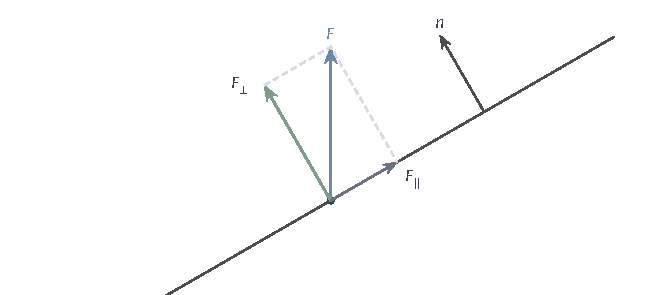
\includegraphics[width=112mm]{figures/00-shared/mathematical-preliminaries-upper/00-shared/tikz/chapter3-concept-processes/normal-projection.pdf}
 \caption{黑斜线表示局部切平面的一个截面，$n$为所选单位法向。向量$F$分为$F_\perp=(F^\top n)n$与切向部分$F_\parallel$；通量使用有符号标量$F^\top n$乘面积，切向部分不贡献。将$n$改为$-n$时标量分量变号，但投影向量$F_\perp$不变，这与直接把场反向不同。}
 \label{fig:analysis-process-normal-projection}
\end{figure}

\paragraph{可积性的要求}

通量只累计法向分量，因此在法向分量可测的前提下，其有限可积性的准确条件是
\[
 \iint_E
 \left|\bm F(\bm r(u,v))^\top(\bm r_u\times\bm r_v)\right|
 \,\mathrm du\,\mathrm dv<\infty.
\]
一个更容易验证的充分条件是$\int_S\lVert\bm F\rVert_2\,\mathrm dS<\infty$：
因为$\lVert\bm n\rVert_2=1$，Cauchy--Schwarz不等式给出
$|\bm F^\top\bm n|\leq\lVert\bm F\rVert_2$，即法向分量不会超过场的大小。
连续向量场在本节的紧致有限分片曲面上有界，因而满足这一充分条件。

反过来，法向分量可积并不要求场的大小可积，因为切向分量再大也不进入通量。

\begin{example}[切向场大小不可积而通量为零]
\label{ex:analysis-tangential-field-zero-flux}
设$S=\{(x,y,0)^\top:x^2+y^2\leq1\}$是平面$z=0$上的单位圆盘，用参数$\bm r(x,y)=(x,y,0)^\top$，则$J_S=1$；取向上法向$\bm n=(0,0,1)^\top$。
令$\bm F(\bm x)=(\lVert\bm x\rVert_2^{-2},0,0)^\top$，原点处任取一值。
由极坐标换元（示例~\ref{ex:analysis-polar-coordinate-jacobian}），
\[
 \int_S\lVert\bm F\rVert_2\,\mathrm dS
 =\int_0^{2\pi}\int_0^1r^{-2}\cdot r\,\mathrm dr\,\mathrm d\theta
 =+\infty,
\]
所以场的大小不可积。
但$\bm F$平行于圆盘，$\bm F^\top\bm n=0$处处成立，法向分量可积，通量为$0$。
\end{example}

这个场的第一个分量在圆盘上不可积，通量却有定义。
所以不能把法向分量可积与向量场各分量都可积视为同一个条件。

\subsubsection{积分的性质}

以下运算都在同一曲面、同一法向约定下进行，并假定各法向分量可积。
它们大多可归结为标量函数$\bm F^\top\bm n$的面积积分，直接沿用第一类积分的性质；与方向有关的法向反转和重参数化则需要单独说明。

\paragraph{加法}

向量场相加以后，其法向分量也相加，因此
\[
 \begin{aligned}
 \int_S(\bm F+\bm G)^\top\bm n\,\mathrm dS
 &=\int_S\bm F^\top\bm n\,\mathrm dS\\
 &\quad{}+\int_S\bm G^\top\bm n\,\mathrm dS.
 \end{aligned}
\]
绝对可积性由两项法向分量的绝对值之和控制，积分等式来自标量面积积分的加法性质。
物理上，两股水流叠加后穿过网的水量，等于两股水流分别穿过的水量之和。

\paragraph{减法}

向量场相减以后，其法向分量也相减，因此
\[
 \begin{aligned}
 \int_S(\bm F-\bm G)^\top\bm n\,\mathrm dS
 &=\int_S\bm F^\top\bm n\,\mathrm dS\\
 &\quad{}-\int_S\bm G^\top\bm n\,\mathrm dS.
 \end{aligned}
\]
两项法向分量绝对可积时，它们的差仍绝对可积，积分等式来自标量面积积分的减法性质。

\paragraph{数乘}

对实数$c$，由$(c\bm F)^\top\bm n=c(\bm F^\top\bm n)$，常数可以提出积分号：
\[
 \int_S(c\bm F)^\top\bm n\,\mathrm dS
 =c\int_S\bm F^\top\bm n\,\mathrm dS.
\]
这里缩放的是场，曲面的法向约定保持固定：流速加倍，穿过的水量也加倍。

\paragraph{曲面分割的可加性}

将$S$分为内部不重叠的有限片$S_1,\ldots,S_N$，并在每片采用原定向的限制，则
\[
 \int_S\bm F^\top\bm n\,\mathrm dS
 =\sum_{j=1}^N\int_{S_j}\bm F^\top\bm n\,\mathrm dS.
\]
零面积接缝不贡献积分。
关键在于每片沿用原来的法向：若某片单独反转法向，这一片计入的是反方向的穿越量，加起来就不再是整张曲面的通量。

\paragraph{法向反转}

在场和曲面不变时，把$\bm n$换成$-\bm n$会使通量变号：
\[
 \int_S\bm F^\top(-\bm n)\,\mathrm dS
 =-\int_S\bm F^\top\bm n\,\mathrm dS.
\]
水流本身没有变，变的只是计数方向：例如原法向朝上时，从下往上的穿越原来记为正，现在记为负。
这与第一类积分不同，后者不使用法向，换定向不改变结果。

\paragraph{重参数化}

更换参数时，所选的几何法向保持不变。
由定理~\ref{thm:analysis-surface-reparameterization}，新参数的叉积等于原叉积乘$\det\bm J_T$，
而二维换元公式使用的是$|\det\bm J_T|$。若$\det\bm J_T>0$，两者相同，式~\eqref{eq:analysis-surface-flux}右端不变；
若$\det\bm J_T<0$，例如交换两个参数，新叉积指向相反一侧，按定义中“方向相反时乘$-1$”的约定校正后，结果仍不变。
因此在固定曲面定向并完成这一校正后，通量只依赖曲面、定向和场，与参数选择无关。

\subsubsection{积分的计算}

计算通量分三步：先确定要用哪一侧的法向，再选一个叉积指向该侧的参数化（若指向相反，就在结果前加负号），最后在参数域上累计$\bm F$与有向面积元的内积。

对于图像曲面$z=\psi(x,y)$，第一类积分的计算中已经求出叉积
\[
 \bm r_x\times\bm r_y=(-\psi_x,-\psi_y,1)^\top,
\]
它的第三分量为正，指向上方。
因此取向上法向时，对$\bm F=(P,Q,R)^\top$有
\[
 \int_S\bm F^\top\bm n\,\mathrm dS
 =\iint_D(-P\psi_x-Q\psi_y+R)(x,y,\psi(x,y))\,\mathrm dx\,\mathrm dy.
\]
取向下法向则在右侧加负号。这一式直接使用有向面积元，叉积的长度已经与单位法向的分母抵消，不能再额外乘一次$\sqrt{1+\psi_x^2+\psi_y^2}$。

斜平面片是$\psi(x,y)=x+y$在单位正方形上的图像，可以用它核对通量与投影面积的关系。

\begin{example}[竖直单位场穿过斜平面片]
\label{ex:analysis-tilted-plane-flux}
取斜平面片$\bm r(u,v)=(u,v,u+v)^\top$、$E=[0,1]^2$和向上单位法向$(-1,-1,1)^\top/\sqrt3$。
对竖直单位场$\bm F=(0,0,1)^\top$，场与参数叉积$(-1,-1,1)^\top$的内积为$1$，故
\[
 \int_S\bm F^\top\bm n\,\mathrm dS
 =\int_0^1\int_0^1 1\,\mathrm du\,\mathrm dv=1.
\]
用面积测度分开看：这块面的面积为$\sqrt3$（示例~\ref{ex:analysis-tilted-plane-area}），场的法向分量为$\bm F^\top\bm n=1/\sqrt3$，两者相乘为$1$，恰好等于它在$xy$平面上的投影面积。
\end{example}

同样地，平面$z=ax+by+c$在单位圆盘$D$上方的部分对该场的向上通量为$\iint_D1\,\mathrm dx\,\mathrm dy=\pi$，
等于水平投影面积；它的实际面积则为$\pi\sqrt{1+a^2+b^2}$。
这与示例~\ref{ex:analysis-tilted-square-flux}中倾斜屋顶接雨的结果一致：竖直的流只“看见”曲面的水平投影。

对半径为$R$的球面，讨论单位法向量时已算出$(\varphi,\theta)$次序的参数叉积为$R\sin\varphi\,\bm r$，它在参数域内部指向外侧。
下面三个例子都取外法向，依次计算径向场、点源场和恒定场的通量。

\begin{example}[径向场穿过球面]
\label{ex:analysis-radial-field-sphere-flux}
令$\bm F(\bm x)=\bm x/R$。在球面上$\bm F$恰等于外单位法向，$\bm F^\top\bm n=1$，由示例~\ref{ex:analysis-sphere-area}，
\[
 \int_S\bm F^\top\bm n\,\mathrm dS
 =\int_S1\,\mathrm dS=4\pi R^2.
\]
取内法向时通量为$-4\pi R^2$。
\end{example}

这次外向通量与面积相等，是因为法向分量处处为$1$。
一般情形下$|\bm F^\top\bm n|\leq\lVert\bm F\rVert_2$，通量的绝对值不超过场的大小对面积的积分；场的方向偏离法向时，只有法向分量计入通量。

接下来的两个例子形成对比：一个场由原点处的点源发出，另一个场在空间中处处相同。

\begin{example}[点源场的通量与半径无关]
\label{ex:analysis-point-source-sphere-flux}
令$\bm F(\bm x)=\bm x/\lVert\bm x\rVert_2^3$（$\bm x\neq\bm0$），$S$是以原点为中心、半径为$R$的球面，外法向为$\bm n=\bm x/R$。
$\bm F$在不含原点的球面上连续，因而法向分量可积。
在$S$上$\lVert\bm x\rVert_2=R$，故
\[
 \bm F^\top\bm n=\frac{\bm x^\top\bm x}{R^3\cdot R}=\frac1{R^2},
\]
外向通量为$(1/R^2)\cdot4\pi R^2=4\pi$。
\end{example}

球面越大，场越弱，但面积增大的倍数恰好抵消场的减弱，所以通量不随$R$改变：
以点源为中心的球面无论多大，测得的点源单位时间放出的总量都一样。

\begin{example}[恒定场穿过球面的净通量为零]
\label{ex:analysis-constant-field-sphere-flux}
令$\bm F=(0,0,1)^\top$。由$\bm r_\varphi\times\bm r_\theta=R\sin\varphi\,\bm r$，被积函数为
$\bm F^\top(\bm r_\varphi\times\bm r_\theta)=R\sin\varphi\cdot R\cos\varphi=R^2\sin\varphi\cos\varphi$，于是
\[
 \int_S\bm F^\top\bm n\,\mathrm dS
 =\int_0^{2\pi}\int_0^\pi R^2\sin\varphi\cos\varphi\,\mathrm d\varphi\,\mathrm d\theta=0.
\]
分开计算，上半球面$0\leq\varphi\leq\pi/2$的外向通量为
\[
 2\pi R^2\int_0^{\pi/2}\sin\varphi\cos\varphi\,\mathrm d\varphi=\pi R^2,
\]
下半球面$\pi/2\leq\varphi\leq\pi$的外向通量为$-\pi R^2$。
\end{example}

在恒定场中，水从下半球面流入球内，又从上半球面等量流出，球内既不产生也不吸收水，所以闭曲面的净通量为零。
包围点源的球面则有正的净通量。
可见闭曲面的净通量反映它所围区域内部的源与汇；
第~\ref{sec:multivariable-boundary-relations}节将用区域内部的散度累计来计算闭曲面的通量，并核对这里的几个结果。

\FloatBarrier
